 \begin{savequote}[8cm]
\textlatin{Cor animalium, fundamentum e\longs t vitæ, princeps omnium, Microco\longs mi Sol, a quo omnis vegetatio dependet, vigor omnis \& robur emanat.}

The heart of animals is the foundation of their life, the sovereign of everything within them, the sun of their microcosm, that upon which all growth depends, from which all power proceeds.
  \qauthor{--- William Harvey \cite{harvey_exercitatio_1628}}
\end{savequote}

\chapter{\label{app:newtech}New Reconstruction Technical Details}

\minitoc

\section{Track number cuts in pioon trackless selection}
\label{sec:app-tlpi-trknumcut}
There are a few track number variables that are helpful in reducing background events for the $\numuccopi$ selection. 
These are:
\begin{enumerate}
    \item $N_{\textrm{tot}}$, The total number of reconstructed tracks.
    \item $N_{\textrm{S-tot}}$, The total number of reconstructed tracks that have a segment in SFGD.
    \item $N_{\textrm{delayed}}$, The number of long delayed tracks.
    \item $N_{\textrm{pri}}$, The number of primary tracks.
    \item $N_{\textrm{non-pri}}$, The number of non-primary tracks.
    \item $N_{\textrm{lone}}$, The number of lone tracks.
    \item $N_{\textrm{gen}}$, The number of generations.
\end{enumerate}
A common feature for these track numbers is that they should not be too large, which should correspond to DIS events.
Hence, a upper cut is implemented on them.
Furthermore, a lower cut, $N_{\textrm{S-tot}}>2$, is useful in cutting away OOFV backgrounds for the TPC-$\mu$ sample.
This is understandable as a $\numuccopi$ event should have the primary muon, the primary pion and most likely, the primary proton as well, thereby leading to at least $3$ reconstructed tracks in SFGD.
As for the SFGD-$\mu$ event, additional lower cuts on  $N_{\textrm{delayed}}$, $N_{\textrm{pri}}$ and $N_{\textrm{tot}}$ are effective in removing CC$0\pi$ backgrounds.
The presence of the CC$0\pi$ background could be due to the mis-identification of a proton track as a muon track and the ME from the muon is mis-identified as the ME from the pion.
These events are likely to have only fewer primary tracks and total number of tracks, so lower cuts on these track number could help to remove such backgrounds.

\begin{figure}
  \centering
  \begin{subfigure}{\dbfigwid\textwidth}
       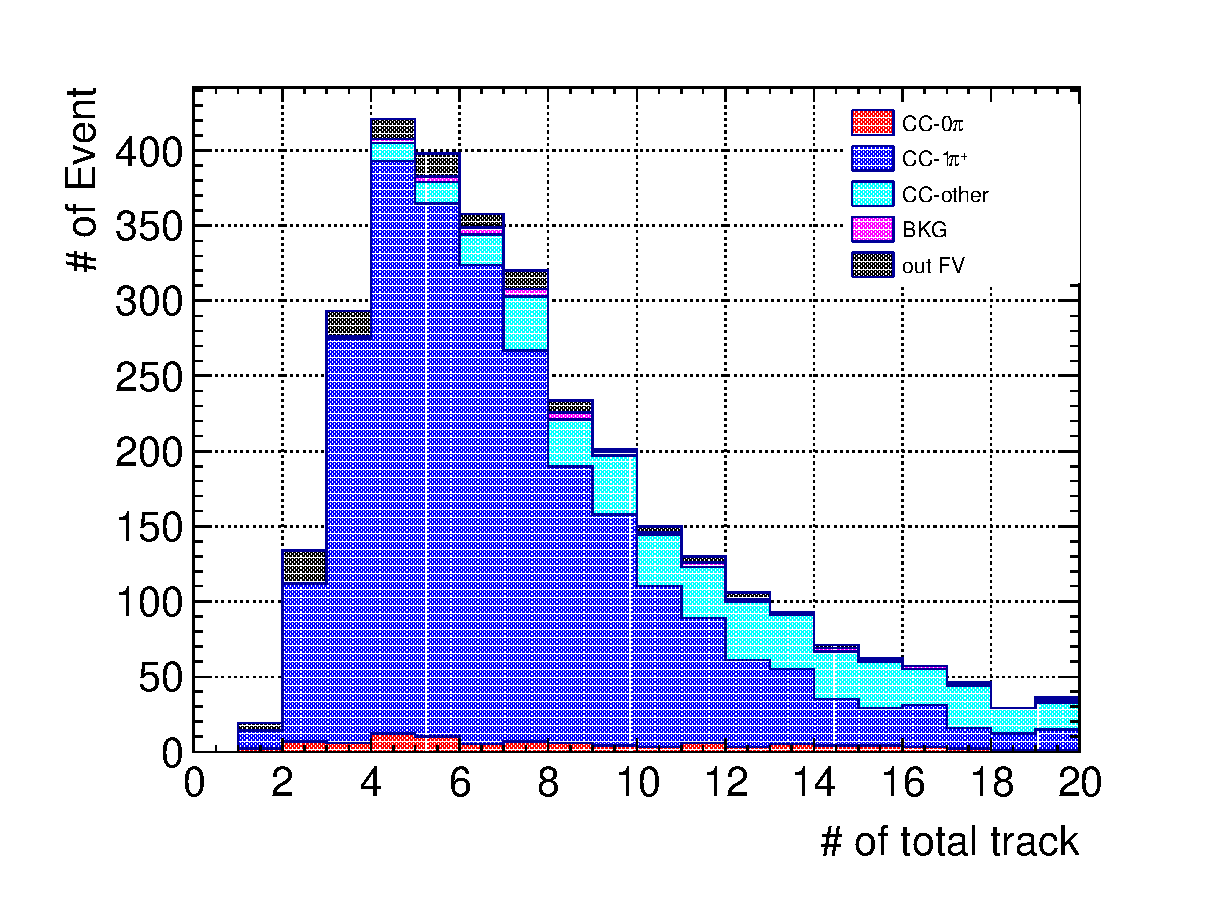
\includegraphics[width=\textwidth]{figures/sel/TPCmu_ntotaltrk_stack_al8.eps}
       \caption{The total number of tracks in the event.}
       \label{subfig:tlpi-trknum-tot}
  \end{subfigure}
  \begin{subfigure}{\dbfigwid\textwidth}
       \includegraphics[width=\textwidth]{figures/sel/TPCmu_nsfgtrk_stack_al8.eps}
       \caption{The total number of tracks with a segment in SFGD.}
       \label{subfig:tlpi-trknum-sfgd}
  \end{subfigure}
  \\
  \begin{subfigure}{\dbfigwid\textwidth}
       \includegraphics[width=\textwidth]{figures/sel/TPCmu_nsdptrk_stack_al8.eps}
       \caption{The number of delayed tracks.}
       \label{subfig:tlpi-trknum-delayed}
  \end{subfigure}
  \begin{subfigure}{\dbfigwid\textwidth}
       \includegraphics[width=\textwidth]{figures/sel/TPCmu_npri_stack_al8.eps}
       \caption{The number of primary tracks.}
       \label{subfig:tlpi-trknum-pri}
  \end{subfigure}
  \\
  \begin{subfigure}{\dbfigwid\textwidth}
       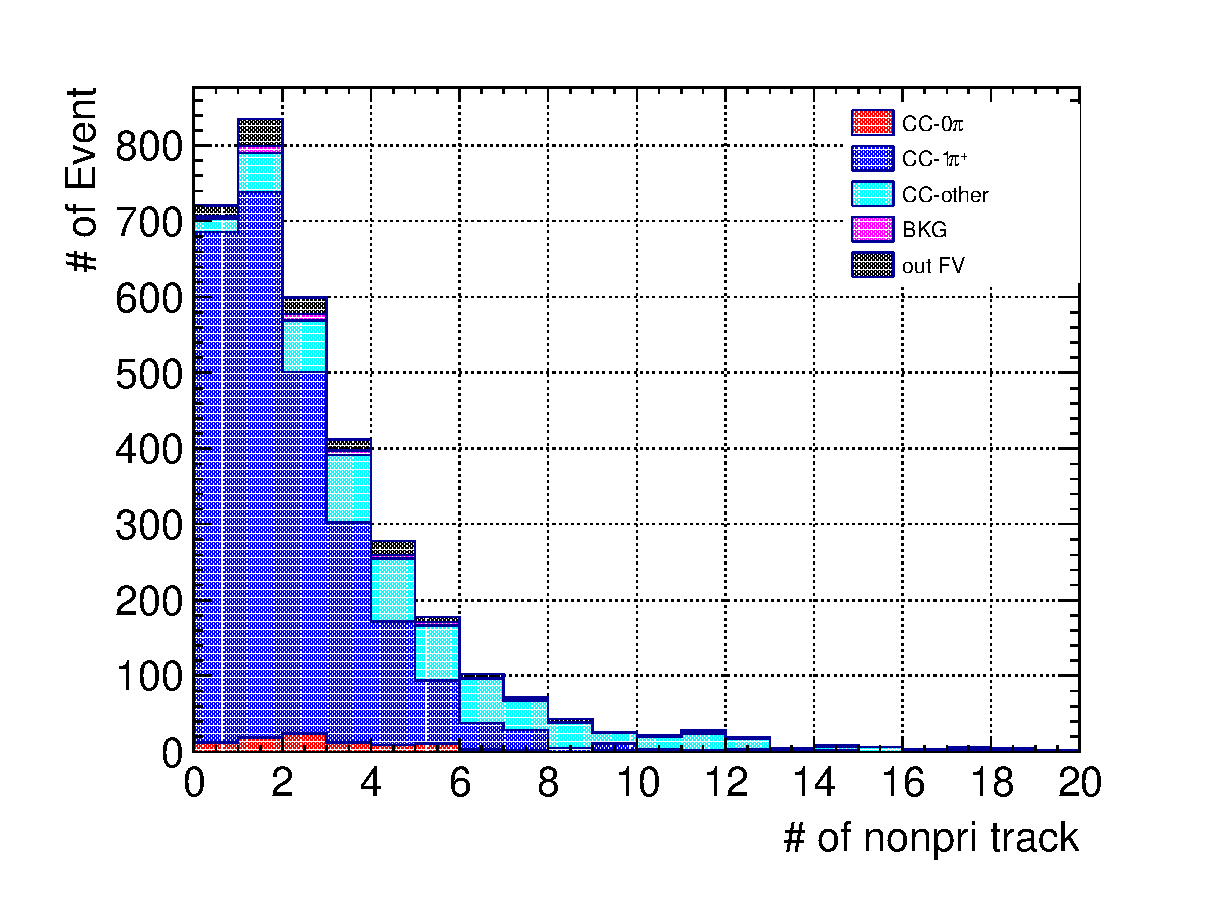
\includegraphics[width=\textwidth]{figures/sel/TPCmu_nnonpritrk_stack_al8.eps}
       \caption{The number of non-primary tracks.}
       \label{subfig:tlpi-trknum-nonpri}
  \end{subfigure}
  \begin{subfigure}{\dbfigwid\textwidth}
       \includegraphics[width=\textwidth]{figures/sel/TPCmu_nlon_stack_al8.eps}
       \caption{The number of lone tracks.}
       \label{subfig:tlpi-trknum-lone}
  \end{subfigure}
  \\
  \begin{subfigure}{\dbfigwid\textwidth}
       \includegraphics[width=\textwidth]{figures/sel/TPCmu_ngen_stack_al8.eps}
       \caption{The number of generations.}
       \label{subfig:tlpi-trknum-gen}
  \end{subfigure}
  \begin{subfigure}{\dbfigwid\textwidth}
       \includegraphics[width=\textwidth]{figures/sel/TPCmu_p_pi_stack_al8.eps}
       \caption{The total number of tracks in the event.}
       \label{subfig:tlpi-trknum-ppi}
  \end{subfigure}
  \caption{Track number distributions for the TPC-$\mu$ sample.}
  \label{fig:tlpi-trknum-tpcmu}
\end{figure}

Fig.~\ref{fig:tlpi-trknum-tpcmu} shows the distributions of the track number variables for the TPC-$\mu$ sub-sample before making any track number cuts.
The selection purity is shown in the topological decomposion of the $\ppi$ distribution in Fig.~\ref{subfig:tlpi-trknum-ppi}.
After some trials and errors and investigating the impact of cuts on a single variable stepwise, the following cuts for the TPC-$\mu$ sub-sample are applied:
\begin{enumerate}
    \item $N_{\textrm{tot}}<12$.
    \item $1<N_{\textrm{S-tot}}<7$.
    \item $N_{\textrm{pri}}<5$.
    \item $N_{\textrm{non-pri}}<5$.
    \item $N_{\textrm{lone}}<5$.
\end{enumerate}
The results of these cuts are shown in Fig.~\ref{fig:tlpi-trknum-tpcmu-cut}.
It turned out that after making the above cuts, further cuts on $N_{\textrm{delayed}}$ and $N_{\textrm{gen}}$ are not necessary.
\begin{figure}
  \centering
  \begin{subfigure}{\dbfigwid\textwidth}
       \includegraphics[width=\textwidth]{figures/sel/TPCmu_ntotaltrk_stack_al9.eps}
       \caption{The total number of tracks in the event.}
       \label{subfig:tlpi-trknum-tot-cut}
  \end{subfigure}
  \begin{subfigure}{\dbfigwid\textwidth}
       \includegraphics[width=\textwidth]{figures/sel/TPCmu_nsfgtrk_stack_al9.eps}
       \caption{The total number of tracks with a segment in SFGD.}
       \label{subfig:tlpi-trknum-sfgd-cut}
  \end{subfigure}
  \\
  \begin{subfigure}{\dbfigwid\textwidth}
       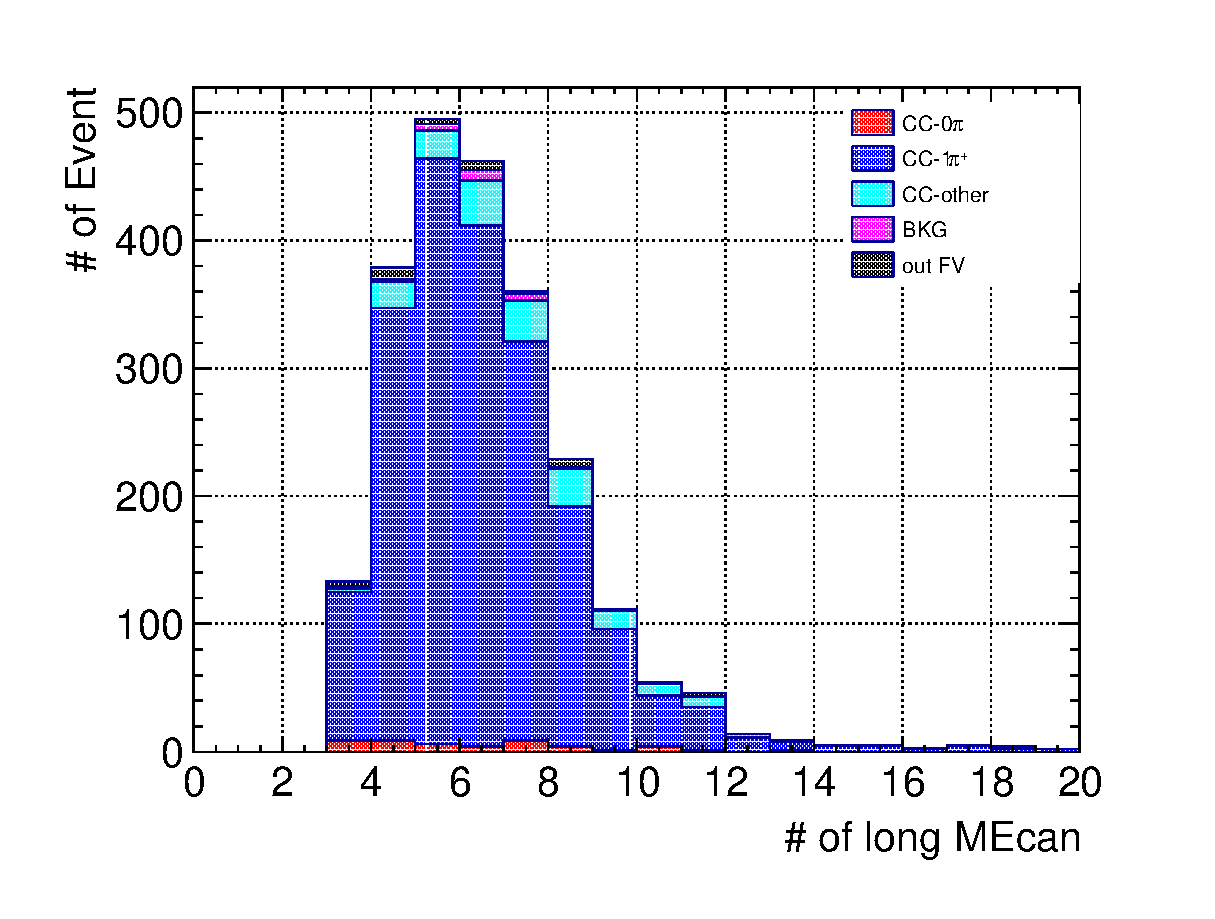
\includegraphics[width=\textwidth]{figures/sel/TPCmu_nsdptrk_stack_al9.eps}
       \caption{The number of delayed tracks.}
       \label{subfig:tlpi-trknum-delayed-cut}
  \end{subfigure}
  \begin{subfigure}{\dbfigwid\textwidth}
       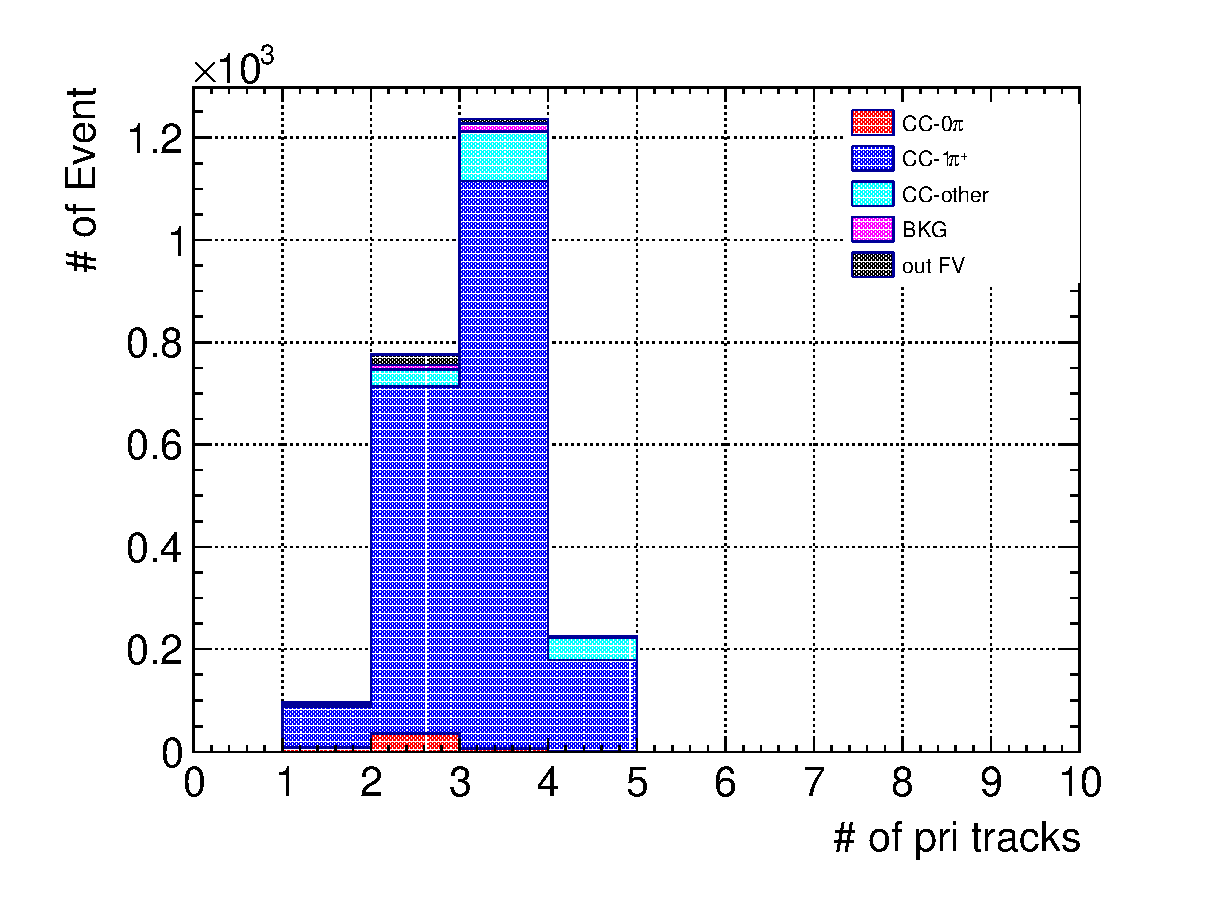
\includegraphics[width=\textwidth]{figures/sel/TPCmu_npri_stack_al9.eps}
       \caption{The number of primary tracks.}
       \label{subfig:tlpi-trknum-pri-cut}
  \end{subfigure}
  \\
  \begin{subfigure}{\dbfigwid\textwidth}
       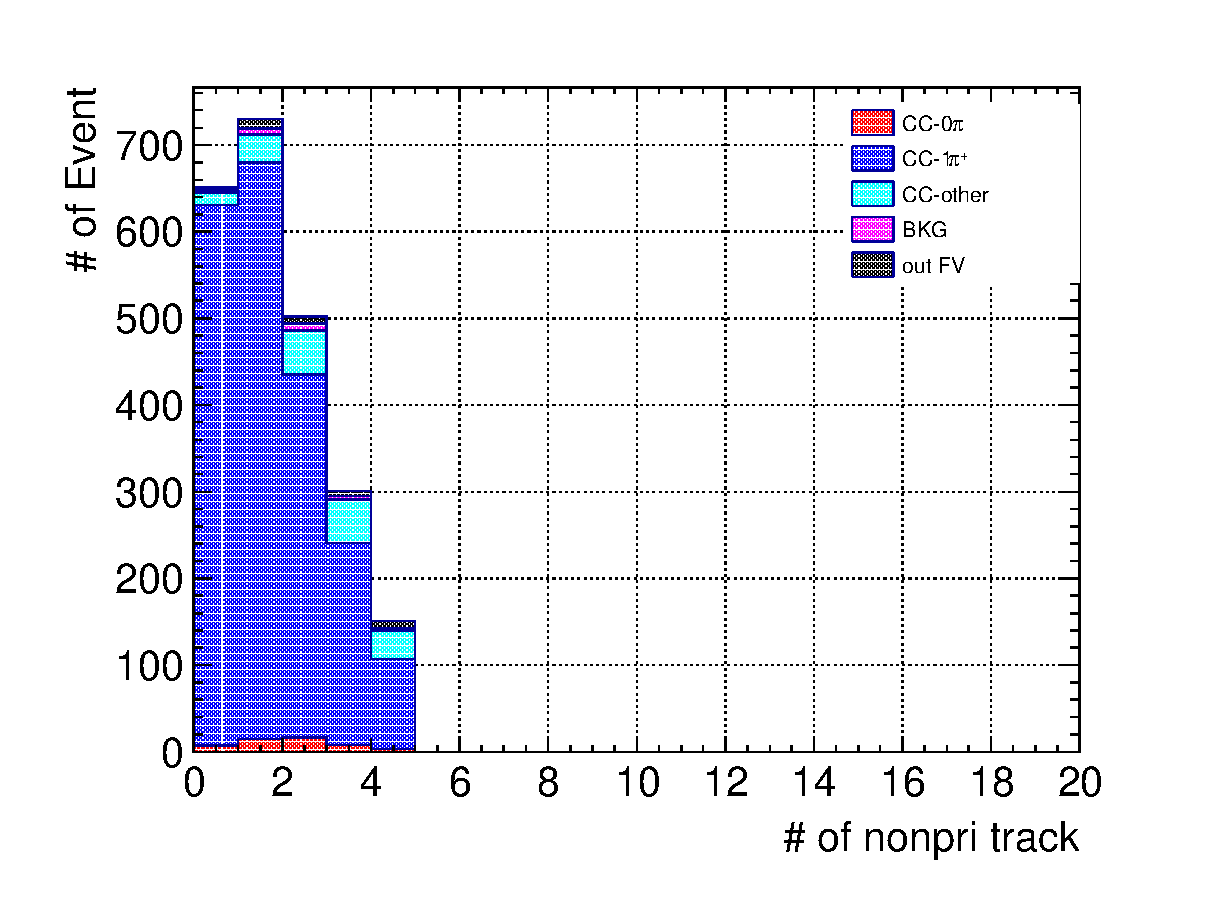
\includegraphics[width=\textwidth]{figures/sel/TPCmu_nnonpritrk_stack_al9.eps}
       \caption{The number of non-primary tracks.}
       \label{subfig:tlpi-trknum-nonpri-cut}
  \end{subfigure}
  \begin{subfigure}{\dbfigwid\textwidth}
       \includegraphics[width=\textwidth]{figures/sel/TPCmu_nlon_stack_al9.eps}
       \caption{The number of lone tracks.}
       \label{subfig:tlpi-trknum-lone-cut}
  \end{subfigure}
  \\
  \begin{subfigure}{\dbfigwid\textwidth}
       \includegraphics[width=\textwidth]{figures/sel/TPCmu_ngen_stack_al9.eps}
       \caption{The number of generations.}
       \label{subfig:tlpi-trknum-gen-cut}
  \end{subfigure}
  \begin{subfigure}{\dbfigwid\textwidth}
       \includegraphics[width=\textwidth]{figures/sel/TPCmu_p_pi_stack_al9.eps}
       \caption{The total number of tracks in the event.}
       \label{subfig:tlpi-trknum-ppi-cut}
  \end{subfigure}
  \caption{Track number distributions for the TPC-$\mu$ sample after making the track number cuts.}
  \label{fig:tlpi-trknum-tpcmu-cut}
\end{figure}
As shown in Fig.~\label{subfig:tlpi-trknum-ppi-cut}, the purity of the $\numuccopi$ selection has improved from $74.1\%$ to $87.5\%$ after making the track number cuts, while the number of signal events decreases from $2496$ to $2044$.
Although the decrease in the signal number is about $18\%$, the remaining number of events is still large enough for the analysis.
The background events are reduced by $66.7\%$ from $874$ to $291$.

A similar investigation is also performed for the SFGD-$\mu$ sub-sample.
The figures before and after the track number cuts are shown in Fig.~\ref{fig:tlpi-trknum-sfgmu} and Fig.~\ref{fig:tlpi-trknum-sfgmu-cut}.
\begin{figure}
  \centering
  \begin{subfigure}{\dbfigwid\textwidth}
       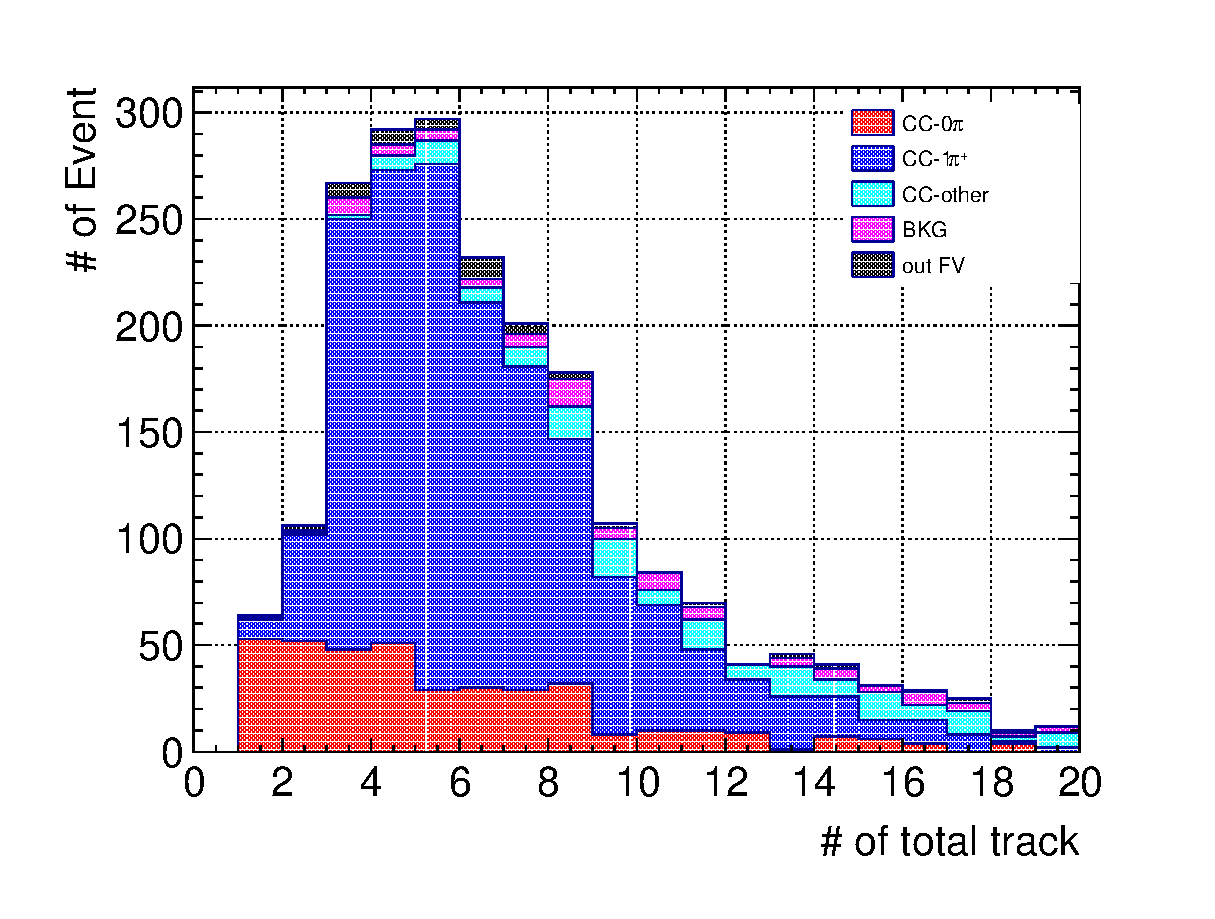
\includegraphics[width=\textwidth]{figures/sel/SFGmu_ntotaltrk_stack_al8.eps}
       \caption{The total number of tracks in the event.}
       \label{subfig:tlpi-trknum-tot-sfgmu}
  \end{subfigure}
  \begin{subfigure}{\dbfigwid\textwidth}
       \includegraphics[width=\textwidth]{figures/sel/SFGmu_nsfgtrk_stack_al8.eps}
       \caption{The total number of tracks with a segment in SFGD.}
       \label{subfig:tlpi-trknum-sfgd-sfgmu}
  \end{subfigure}
  \\
  \begin{subfigure}{\dbfigwid\textwidth}
       \includegraphics[width=\textwidth]{figures/sel/SFGmu_nsdptrk_stack_al8.eps}
       \caption{The number of delayed tracks.}
       \label{subfig:tlpi-trknum-delayed-sfgmu}
  \end{subfigure}
  \begin{subfigure}{\dbfigwid\textwidth}
       \includegraphics[width=\textwidth]{figures/sel/SFGmu_npri_stack_al8.eps}
       \caption{The number of primary tracks.}
       \label{subfig:tlpi-trknum-pri-sfgmu}
  \end{subfigure}
  \\
  \begin{subfigure}{\dbfigwid\textwidth}
       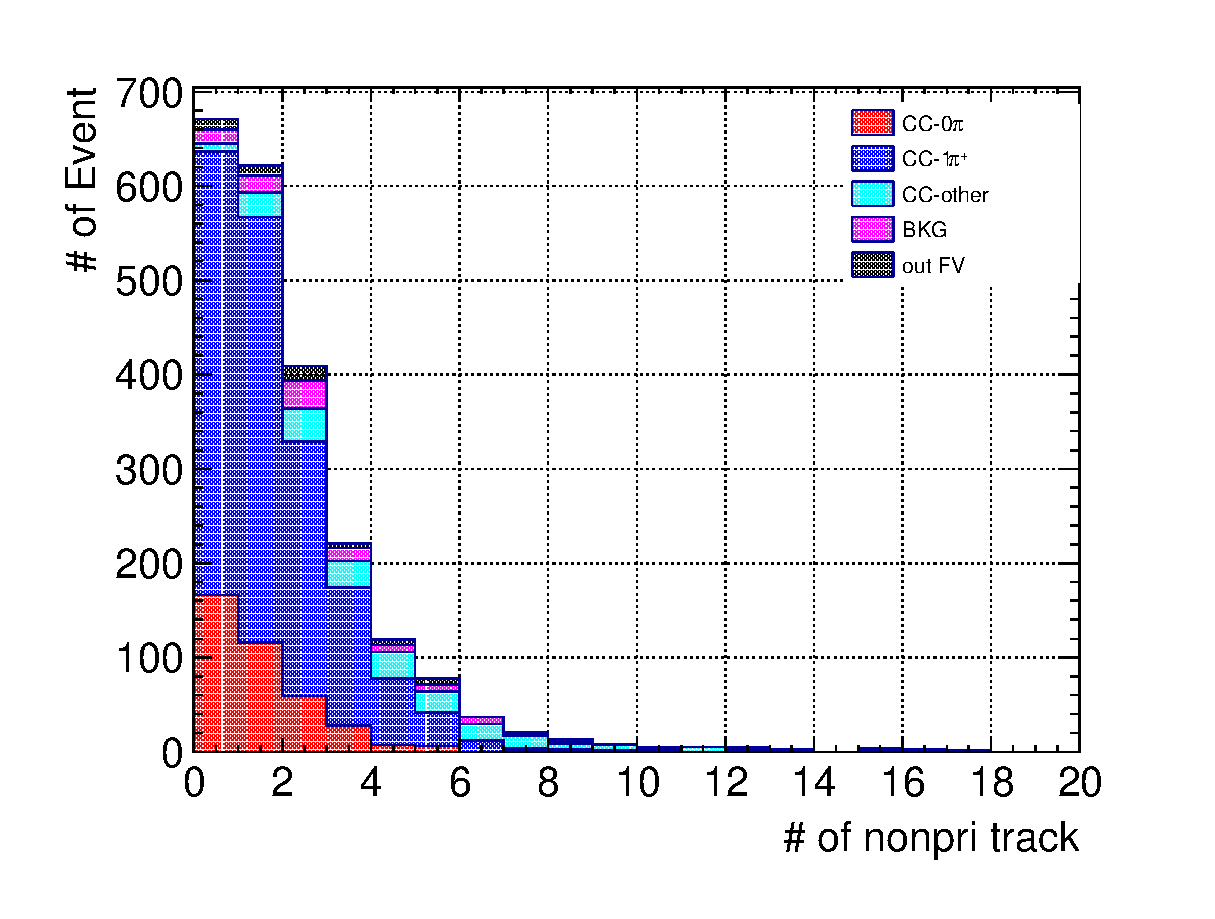
\includegraphics[width=\textwidth]{figures/sel/SFGmu_nnonpritrk_stack_al8.eps}
       \caption{The number of non-primary tracks.}
       \label{subfig:tlpi-trknum-nonpri-sfgmu}
  \end{subfigure}
  \begin{subfigure}{\dbfigwid\textwidth}
       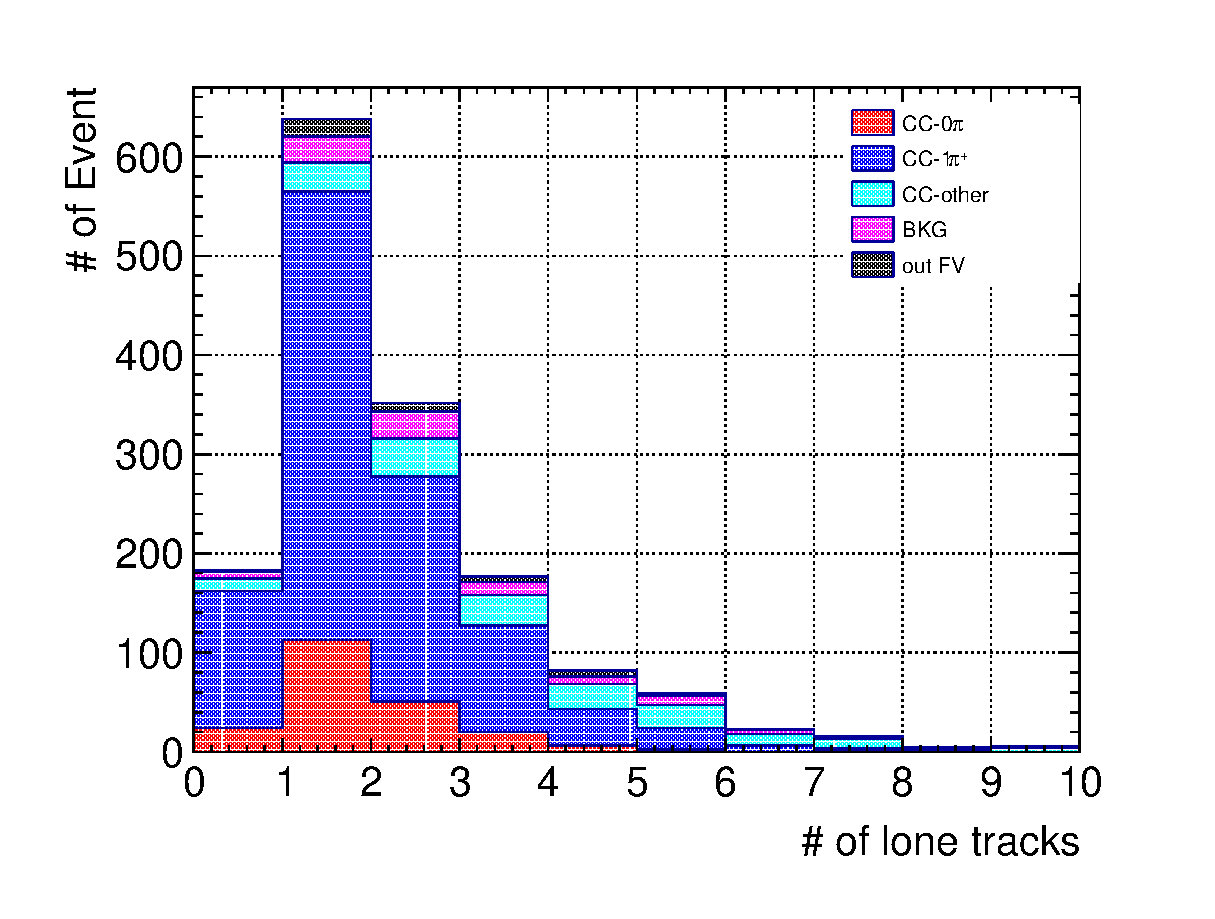
\includegraphics[width=\textwidth]{figures/sel/SFGmu_nlon_stack_al8.eps}
       \caption{The number of lone tracks.}
       \label{subfig:tlpi-trknum-lone-sfgmu}
  \end{subfigure}
  \\
  \begin{subfigure}{\dbfigwid\textwidth}
       \includegraphics[width=\textwidth]{figures/sel/SFGmu_ngen_stack_al8.eps}
        \caption{The number of generations.}
        \label{subfig:tlpi-trknum-gen-sfgmu}
  \end{subfigure}
  \begin{subfigure}{\dbfigwid\textwidth}
       \includegraphics[width=\textwidth]{figures/sel/SFGmu_p_pi_stack_al8.eps}
       \caption{The total number of tracks in the event.}
       \label{subfig:tlpi-trknum-ppi-sfgmu}
  \end{subfigure}
  \caption{Track number distributions for the SFGD-$\mu$ sample.}
  \label{fig:tlpi-trknum-sfgmu}
\end{figure}

\begin{figure}
  \centering
  \begin{subfigure}{\dbfigwid\textwidth}
       \includegraphics[width=\textwidth]{figures/sel/SFGmu_ntotaltrk_stack_al9.eps}
       \caption{The total number of tracks in the event.}
       \label{subfig:tlpi-trknum-tot-sfgmu-cut}
  \end{subfigure}
  \begin{subfigure}{\dbfigwid\textwidth}
       \includegraphics[width=\textwidth]{figures/sel/SFGmu_nsfgtrk_stack_al9.eps}
       \caption{The total number of tracks with a segment in SFGD.}
       \label{subfig:tlpi-trknum-sfgd-sfgmu-cut}
  \end{subfigure}
  \\
  \begin{subfigure}{\dbfigwid\textwidth}
       \includegraphics[width=\textwidth]{figures/sel/SFGmu_nsdptrk_stack_al9.eps}
       \caption{The number of delayed tracks.}
       \label{subfig:tlpi-trknum-delayed-sfgmu-cut}
  \end{subfigure}
  \begin{subfigure}{\dbfigwid\textwidth}
       \includegraphics[width=\textwidth]{figures/sel/SFGmu_npri_stack_al9.eps}
       \caption{The number of primary tracks.}
       \label{subfig:tlpi-trknum-pri-sfgmu-cut}
  \end{subfigure}
  \\
  \begin{subfigure}{\dbfigwid\textwidth}
       \includegraphics[width=\textwidth]{figures/sel/SFGmu_nnonpritrk_stack_al9.eps}
       \caption{The number of non-primary tracks.}
       \label{subfig:tlpi-trknum-nonpri-sfgmu-cut}
  \end{subfigure}
  \begin{subfigure}{\dbfigwid\textwidth}
       \includegraphics[width=\textwidth]{figures/sel/SFGmu_nlon_stack_al9.eps}
       \caption{The number of lone tracks.}
       \label{subfig:tlpi-trknum-lone-sfgmu-cut}
  \end{subfigure}
  \\
  \begin{subfigure}{\dbfigwid\textwidth}
       \includegraphics[width=\textwidth]{figures/sel/SFGmu_ngen_stack_al9.eps}
       \caption{The number of generations.}
       \label{subfig:tlpi-trknum-gen-sfgmu-cut}
  \end{subfigure}
  \begin{subfigure}{\dbfigwid\textwidth}
       \includegraphics[width=\textwidth]{figures/sel/SFGmu_p_pi_stack_al9.eps}
       \caption{The total number of tracks in the event.}
       \label{subfig:tlpi-trknum-ppi-sfgmu-cut}
  \end{subfigure}
  \caption{Track number distributions for the SFGD-$\mu$ sample after making the track number cuts.}
  \label{fig:tlpi-trknum-sfgmu-cut}
\end{figure}
The cuts for the SFGD-$\mu$ sub-sample are:
\begin{enumerate}
    \item $1<N_{\textrm{tot}}<15$.
    \item $1<N_{\textrm{S-tot}}<7$.
    \item $N_{\textrm{delayed}}>4$.
    \item $1<N_{\textrm{pri}}<6$.
    \item $N_{\textrm{non-pri}}<6$.
    \item $N_{\textrm{lone}}<6$.
    \item $N_{\textrm{gen}}<3$.
\end{enumerate}
The purity for this sub-sample has improved from $65.9\%$ to $80.7\%$ after making the track number cuts, while the number of signal events decreases from $1464$ to $1257$, corresponding to a $14.1\%$.
The background events are reduced by $60.3\%$ from $758$ to $301$.

\section{Pull distributions for the stopping pion bottom HAT sub-sample}
\label{sec:app-bot-pulls}
The final distributions of the pull variables and the heavy length for the stopping pion bottom HAT sub-sample are shown in Figure~\ref{fig:app-pulls-res-bot}.
It demonstrates that the applied cuts for these variables are near optimal.
A stricter cut could be put on the heavy length, but this finer cut is not necessary at this stage as the HAT reconstruction and the global matching are still being improved.
\begin{figure}
  \centering
  \begin{subfigure}{\dbfigwid\textwidth}
       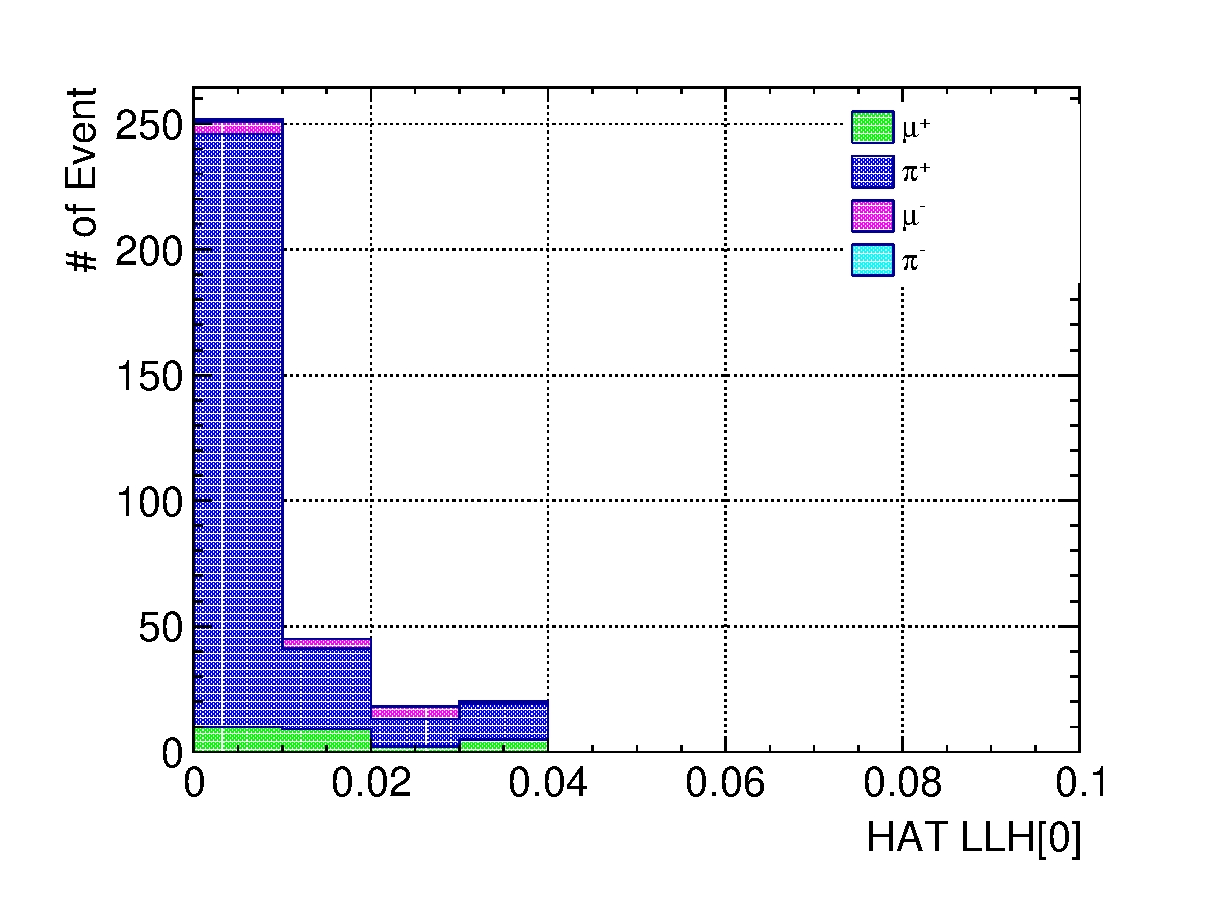
\includegraphics[width=\textwidth]{figures/sel/sspi_BOT_hat_pid0_stack_al6_zoom.eps}
       \caption{The first pull.}
       \label{subfig:sppi-pulls-1-res-bot}
  \end{subfigure}
  \begin{subfigure}{\dbfigwid\textwidth}
       \includegraphics[width=\textwidth]{figures/sel/sspi_BOT_hat_pid1_stack_al6_zoom.eps}
       \caption{The second pull.}
       \label{subfig:sppi-pulls-2-res-bot}
  \end{subfigure}
  \\
  \begin{subfigure}{\dbfigwid\textwidth}
       \includegraphics[width=\textwidth]{figures/sel/sspi_BOT_hat_pid3_stack_al6_zoom.eps}
       \caption{The fourth pull.}
       \label{subfig:sppi-pulls-4-res-bot}
  \end{subfigure}
  \begin{subfigure}{\dbfigwid\textwidth}
       \includegraphics[width=\textwidth]{figures/sel/sspi_BOT_trk_heavylen_stack_al6_zoom.eps}
       \caption{Heavy length.}
       \label{subfig:sppi-heavylen-res-bot}
  \end{subfigure}
  \caption{Pull distributions and a distrution of heavy length at HAT with a cut on the first pull.}
  \label{fig:app-pulls-res-bot}
\end{figure}